\section{The Source of Approximation Bias}
\label{sec:source-of-bias}

To calculate an estimate of $f_i$, the level $w_i^*$ is chosen by Kmerlight
to maximize $t_i^{(w)}$ -- the number of collision-free counters with value $i$ at level $w$.

$$t_i^{(w)} = |\{T_w[c].v = i ~|~ c \in \{0, \dots, r-1\}\}| 
~~~~~~~~~~~~ w_i^* = \arg\max_w t_i^{(w)}$$

Then the number of counters at this level is converted into the estimate of
$f_i$ by multiplying it by $2^{w^*_i} \cdot \left(1 - \frac{1}{r}\right)^{1 - F_0/2^{w^*_i}}$. 

The reason for selecting level $w_i^*$ by this criterion 
is not clearly stated in Kmerlight's original paper \cite{Sivadasan2016}. 
We believe that the authors hoped to minimize the variance of the estimator $\hat f_i$
by including as many $k$-mers in the estimate as possible.

\subsection{Analytical $w^+$}
\label{sec:analytical-w}
In order to get insight into which levels $w_i^*$ are selected by Kmerlight, 
we will analytically find the levels $w_i^+$ that maximize $E(t_i^{(w)})$ -- the expected number 
of collison-free counters with value $i$.

As it was derived in (\ref{eq:ti}), 
$E(t_i^{(w)}) = f_i / 2^w \cdot \left(1 - \frac{1}{r}\right)^{F_0/2^w - 1}$.
The value of $w_i^+$ at which $E(t_i^{(w)})$ is maximized can be obtained by differentiation 
($\frac{\mathrm{d}}{\mathrm{d}w}E(t_i^{(w)}) = 0$) or by using the discrete inequalities 
$E(t_i^{(w^+_i-1)}) \leq E(t_i^{(w^+_i)}) \leq E(t_i^{(w^+_i+1)})$. 
By manipulating the inequalities we get
\begin{equation} \label{eq:wplusbounds}
\frac{1}{4} \leq \left(1 - \frac{1}{r}\right)^{F_0/2^{w^+_i}} \leq \frac{1}{2}
\end{equation}
and finally we can caluclate $w_i^+$:
$$\lg F_0 + \lg\lg \frac{r}{r-1}-1 \leq w_i^+ \leq \lg F_0 + \lg\lg \frac{r}{r-1}$$
Symbol $\lg$ denotes the binary logarithm. 

As $w_i^+$ denotes a Kmerlight's level, it should always be a positive integer.
In rare cases there can be two solutiotions $w_i^+ = \lfloor \lg F_0 + \lg\lg \frac{r}{r-1} \rfloor,
w_i^+ = \lceil \lg F_0 + \lg\lg \frac{r}{r-1} \rceil$. For some values of $F_0$ the optimal 
value of $w_i^+$ may be less than one, but in these cases we choose $w_i^+=1$. In practice,
$w^+_i$ can be simply computed by a for-loop through $w=1, \dots, W$, choosing $w$ that
maximizes $E(t_i^{(w)})$. 

\medskip

Note that the choice of the optimal level $w_i^+$ does not depend on values of $i$ or $f_i$,
but only on values of $F_0$ and $r$. Since $w_1^+ = w_2^+ = \dots = w_m^+$, from now on 
we will refer to this level simply by $w^+$.
As the level $w^+$ maximizes $E(t_i^{(w)})$ for any non-zero value $i$, 
this level also maximizes the expected number of all non-empty collision-free counters
$E(t^{(w)}) = \sum_{i=1}^m E(t_i^{(w)}) = F_0 / 2^w \cdot
\left(1 - \frac{1}{r}\right)^{F_0/2^w - 1} $.

% Apart from our ability to calculate $w^*$ and $p_{cf}$, an important outcome of
% this section is the observation that the value $w^*$ selected by Kmerlight should not
% depend on $i$ or $f_i$ and it is expected to be the same for the estimates of all $f_i$.

\subsection{Explanation of Bias}
Since the ratio $f_i / F_0$ is typically very low for higher values of $i$, and this
ratio determines the value of $t_i^{(w)}$ (the number of collision-free counters holding
the value $i$), each $f_i$ is represented by only a relatively small number of collision-free
counters at each level of Kmerlight's sketch. Therefore $t_i^{(w)}$ have high relative variances. 

%The expected number of collision-free counters at level $w$ is 
%$E(t^{(w)}) = r \cdot p_{cf} = F_0 / 2^w \cdot (1 - 1/r)^{F_0/2^w - 1}$ from \ref{eq:pcf}.
%From the bounds \ref{eq:wplusbounds} we know that at level $w^*$
%$1/4 \leq (1 - 1/r)^{F_0/2^{w^*}} \leq 1/2$.

By examining the levels $w^+-1$ and $w^++1$ we learn that the number of collision-free
counters at these levels is similar to the number of collision-free counters at level $w^+$. 
From (\ref{eq:ti}) we can see that there are two times more $k$-mers hashed into the level $w^+-1$
than $k$-mers hashed into $w^+$, but also more collisions happen at $w^+-1$. These
two effects partially cancel each other out and maintain similar values of $E(t^{(w)})$
for $w = w^+-1, w^+, w^++1$.

As we substitute bounds from (\ref{eq:wplusbounds}) into (\ref{eq:ti}), we learn that
$$ 
\frac{F_0}{2^{w^+}} \cdot \frac{1}{4} \cdot \left(1 - \frac{1}{r}\right)^{-1}
\leq E(t^{(w^+)}) \leq 
\frac{F_0}{2^{w^+}} \cdot \frac{1}{2} \cdot \left(1 - \frac{1}{r}\right)^{-1}
$$
and if we do the same for the level $w^+-1$ we get:
$$ 
2 \cdot \frac{F_0}{2^{w^+}} \left(\frac{1}{4}\right)^2 \left(1 - \frac{1}{r}\right)^{-1}
\leq E(t^{(w^+-1)}) \leq 
2 \cdot \frac{F_0}{2^{w^+}} \left(\frac{1}{2}\right)^2 \left(1 - \frac{1}{r}\right)^{-1}
$$
Finally, for the level $w^++1$ we get:
$$ 
\frac{1}{2} \cdot \frac{F_0}{2^{w^+}} \left(\frac{1}{4}\right)^{1/2} \left(1 - \frac{1}{r}\right)^{-1}
\leq E(t^{(w^++1)}) \leq 
\frac{1}{2} \cdot \frac{F_0}{2^{w^+}} \left(\frac{1}{2}\right)^{1/2} \left(1 - \frac{1}{r}\right)^{-1}
$$


If we substitute $c = F_0/2^{w^+} \cdot (1-1/r)^{-1}$,
we can summarize the similarity of levels as follows:
\begin{equation} \label{eq:level-similarity}
E(t^{(w^+)}) \in \left\langle \frac{1}{4}c, \frac{1}{2}c  \right\rangle ~~~~
E(t^{(w^+-1)}) \in \left\langle \frac{1}{8}c, \frac{1}{2}c  \right\rangle ~~~~
E(t^{(w^++1)}) \in \left\langle \frac{1}{4}c,\frac{1}{2\sqrt{2}}c  \right\rangle
\end{equation}

As a result of low values and high variances of $t_i^{(w)}$ and similar
values of $E(t^{(w^+-1)})$, $E(t^{(w^+)})$ and $E(t^{(w^++1)})$, any of these levels could
hold the maximal $t_i^{(w)}$ and become chosen by Kmerlight as its $w^*_i$. 

Kmerlight always chooses the level which maximizes $t_i^{(w)}$ and this freedom of choice 
leads to values of $t_i^{(w^*_i)}$ consistently higher than values of $E(t_i^{(w^+)})$
which consequently biases the estimator $\hat f_i$ towards higher values.

\begin{figure}[h]
\centerline{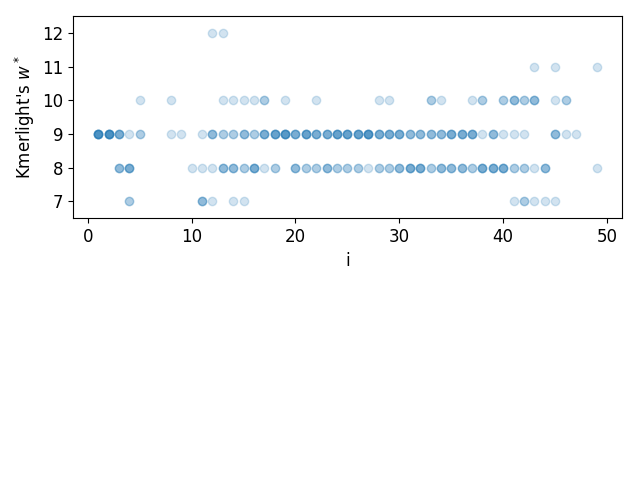
\includegraphics[width=0.75\textwidth, trim={0cm, 5.2cm, 0cm, 0cm}, clip]{images/kmerlight_wstar.png}}
\caption[$w_i^*$ selected by Kmerlight]{Each column 
shows at most seven levels $w_i^*$ that were selected by one of seven instances of Kmerlight.
If a level was chosen by more instances for a specific $i$, its circle is darker.
Kmerlight was run with the same parameters and on the same set of reads as in 
experiment in section \ref{sec:error-characteristics}.}
\label{img:w-selected-by-kmerlight}
\end{figure}

We extracted the values $w_i^*$ for different $f_i$ from one Kmerlight run
and we present them in Figure \ref{img:w-selected-by-kmerlight}.
For each $i$ there are up to seven values of $w_i^*$, each selected by one 
instance of seven Kmerlight's sketches\footnote{If there are no counters holding 
the value $i$ in the whole sketch,  Kmerlight's instance does not choose any level
and estimates $f_i$ as zero.}. The most of selected levels follow the analytical 
$w^+ = 9$; however, Kmerlight often chooses level 8 or 10 to maximize $t_i^{(w)}$. 
Note that for $3\leq i \leq 15$ and $i \geq 40$, the values of $f_i$ are low, and thus 
$t_i^{(w)}$ have high relative variance (as it was presented in section
\ref{sec:error-characteristics}). The maximal $t_i^{(w)}$ can thus also be reached
at levels more distant from the analytical $w^+ = 9$.

\subsection{The Content of Counters}
To provide an insight into the relations presented in (\ref{eq:level-similarity}),
let us now briefly investigate, how the numbers of empty,
collision-free and colliding counters vary acrross levels.

As we focus on a single level $w$, let us denote as $p_{cf}$ the probability
that a single counter is non-empty and collision-free. In other words, $p_{cf}$ is the 
probability that exactly one of $F_0/2^w$ $k$-mers was hashed into that counter.

The number of distinct $k$-mers hashed into one counter ($X$)
follows a binomial distribution, $X \sim \mathrm{Bin}(F_0/2^w, 1/r)$, 
so $p_{cf}$ can be expressed as follows:
\begin{equation} \label{eq:pcf}
p_{cf} = P[X=1] = \frac{F_0}{2^w} \cdot \frac{1}{r} \left(1 - \frac{1}{r}\right)^{F_0/2^w - 1}_{.}
\end{equation}
Similarly, we can derive the probability $p_e$ that a counter is empty and the probability 
$p_c$ that a counter holds a collision:
$$p_e = P[X=0] = \left(1 - \frac{1}{r}\right)^{F_0/2^w} ~~~~~~ p_c = P[X>1] = 1 - p_e - p_{cf}$$

Note that the expected number of non-empty collion-free counters at one level is 
$E(t^{(w)}) = r \cdot p_{cf}$. 

In order to further demonstrate the similarity of $E(t^{(w)})$ at the levels close to $w^+$ we
display the values of $p_{cf} = E(t^{(w)}) / r, p_e, p_c$ for different levels in
Figure \ref{img:pe-pcf-pc}. These probabilities represent the fractions of 
non-empty collision-free, empty and collided counters respectively. 

\begin{figure}[h]
\centerline{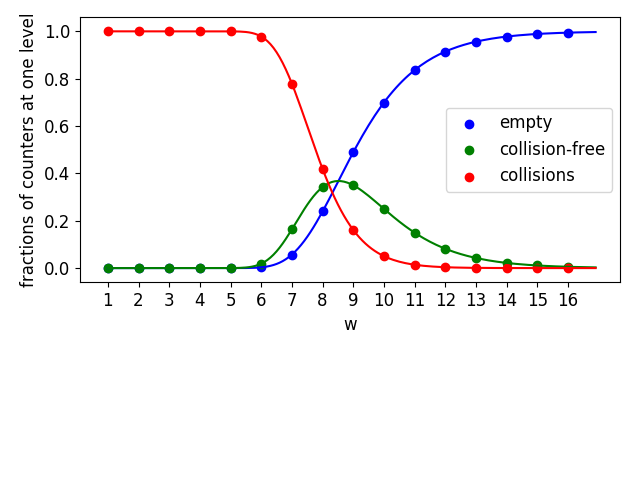
\includegraphics[width=0.8\textwidth, trim={0cm, 3.5cm, 0cm, 0cm}, clip]{images/pcf.png}}
\caption[Plot of $p_e, p_{cf}, p_c$ across the levels]{The values of $p_e, p_{cf}, p_c$ 
represent the theoretical fractions of empty, collision-free and collided counters in
each level respectively. To make these theoretical values comparable to the experimental
resultes from section \ref{sec:error-characteristics}, we set $F_0 = 1.2 \times 10^7, r = 2^{15}$.} 
\label{img:pe-pcf-pc}
\end{figure}

The presented settings show one of the worst possible situations. Since
$E(t^{(8)}) \approx E(t^{(9)})$, Kmerlight very frequently chooses the level $w_i^*$ from 
$\{8, 9\}$ (as it can be seen at Figure \ref{img:w-selected-by-kmerlight}), 
but it always prefers the one with the highest value of $t^{(w)}$.
Thus $E(t_i^{(w^*_i)}) > E(t^{(8)}) \approx E(t^{(9)})$, which results in overestimation.

If there was a greater difference between $E(t^{(w^+)})$, $E(t^{(w^+-1)})$ and
$E(t^{(w^++1)})$, Kmerlight would choose the level $w^+$ much more often than the other
levels and so it would have a smaller chance of choosing $t_i^{(w^*_i)} > E(t^{(w^+)})$.
